\begin{question}
\noindent Triangle $P$ has vertices $A(1,1)$, $B(2,1)$ and $C(1,3)$.

Triangle $P$ is enlarged by scale factor $2$, using centre of enlargement $(0,0)$, to give triangle $P'$.

\begin{center}
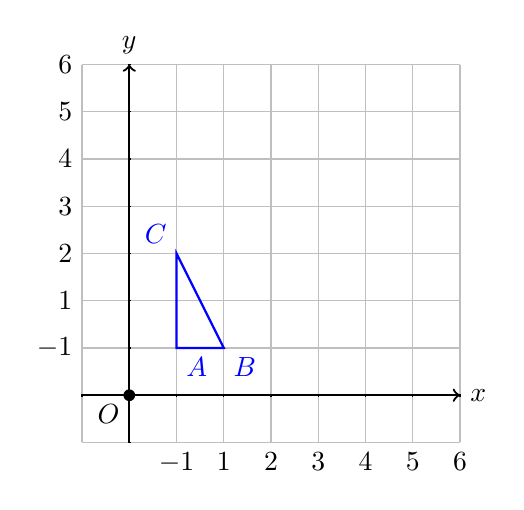
\begin{tikzpicture}[scale=0.6]
    \draw[step=1, lightgray, thin] (-1,-1) grid (7,7);
    \draw[->, thick] (-1,0) -- (7,0) node[right] {$x$};
    \draw[->, thick] (0,-1) -- (0,7) node[above] {$y$};

    \foreach \x in {-1,0,1,2,3,4,5,6,7} \draw (\x,-1pt) -- (\x,1pt);
    \foreach \y in {-1,0,1,2,3,4,5,6,7} \draw (-1pt,\y) -- (1pt,\y);

    \node[below] at (1,-1) {$-1$};
    \node[below] at (2,-1) {$1$};
    \node[below] at (3,-1) {$2$};
    \node[below] at (4,-1) {$3$};
    \node[below] at (5,-1) {$4$};
    \node[below] at (6,-1) {$5$};
    \node[below] at (7,-1) {$6$};

    \node[left] at (-1,1) {$-1$};
    \node[left] at (-1,2) {$1$};
    \node[left] at (-1,3) {$2$};
    \node[left] at (-1,4) {$3$};
    \node[left] at (-1,5) {$4$};
    \node[left] at (-1,6) {$5$};
    \node[left] at (-1,7) {$6$};

    \draw[thick, blue] (1,1) -- (2,1) -- (1,3) -- cycle;
    \node[below right, blue] at (1,1) {$A$};
    \node[below right, blue] at (2,1) {$B$};
    \node[above left, blue] at (1,3) {$C$};

    \node at (0,0) [circle, fill=black, inner sep=1.5pt]{};
    \node[below left] at (0,0) {$O$};
\end{tikzpicture}
\end{center}

\noindent On a copy of this grid, draw and label triangle $P'$, the image of triangle $P$ after the enlargement.

\vspace{5cm}

\begin{flushright}
    \answerplain{3}
\end{flushright}
\end{question}